Proton bunches at the LHC contain approximately $10^{11}$ protons which is necessary to achieve the high luminosities discussed in the prior section. Unfortunately, due to the large number of protons in a proton bunch multiple interactions happen per bunch crossing. During the crossing, there is one primary inelastic hard scattering event, which produces the physics of interest. Additionally, there are many soft scattering collisions, referred to as pileup, which obscure the collision of interest.

As luminosity increases, so does pileup, presenting a trade off between achieving high luminosity and high pileup or low luminosity and low pileup. The physics processes of interest at the LHC are rare, and thus require high luminosity, so efforts are focused on mitigating the resulting pileup. One strategy involves leveraging the granularity of the Inner Detector as described in Section~\ref{sec:atlas_id}, which can help distinguish between the primary interaction and the softer interactions. Additionally, software based techniques used during event reconstruction can help suppress pileup effects, and are further discussed in Chapter~\ref{ch:reco}.
Pileup is quantified by the average number of interactions per bunch crossing, $\langle \mu \rangle$, which is determined from the luminosity block (lb), which is defined as a short interval over which the instantaneous luminosity is approximately constant. The average value of $\langle \mu \rangle$ was 43 in 2022, 51 in 2023, and 58 in 2024~\cite{atlas_pileup_image}. Figure~\ref{fig:atlas_run3_pileup} shows the pileup distributions during the first three years of Run 3.

\begin{figure}
    \centering
    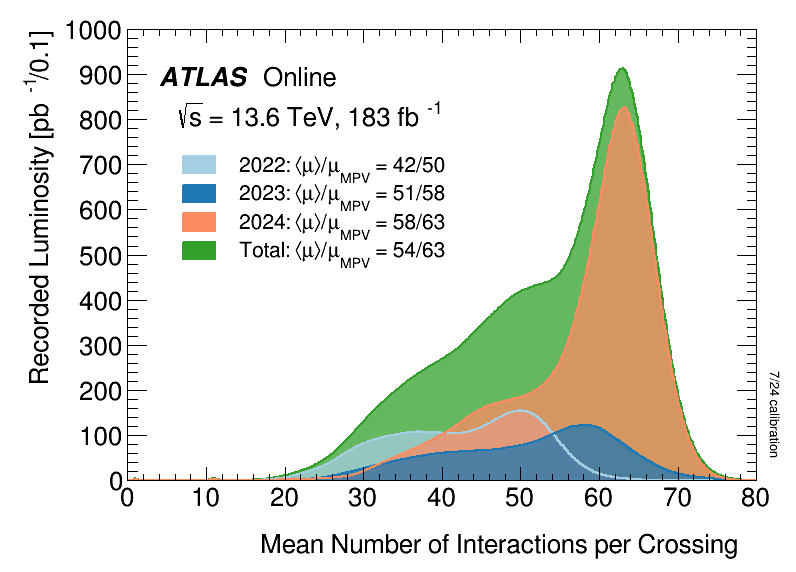
\includegraphics[width=0.8\textwidth]{figures/atlas/atlas_run3_pileup.png}
    \caption{Shown is the luminosity-weighted distribution for the mean number of interactions per bunch crossing for 2022--2024 pp collision data. Taken from~\cite{atlas_pileup_image}}\label{fig:atlas_run3_pileup}
\end{figure}